
\chapter{Optimization}\label{section:optimization}

TODO : Write Introduction

\section{Optimization under Uncertainty}

While some things in life are certain, most are not and this is as true for optimization as for anything else. That means, that while optimizing anything from next years crop to tomorrows energy pricing might be done by assuming fixed values for the parameters of a optimization problem, in reality most of these parameters will contain uncertainty. The field of Stochasitc Programming contains is occupied with finding methods that allow for introducing these uncertainties into optimization problems.

One way to approach these uncertainties is to split the problem in scenarios. A bakery for example has to decide on how many Baguettes to bake for the next day with the objective of maximizing its profit. Baking too little Baguettes will lead to missing out on potential sales while baking too many baguettes will mean that the demand is fullfilled but the money invested in the excess number of baguettes is lost. Assuming the mean number of baguettes bought every day is $1000$, the price to buy a baguette is $1 €$ and the cost to produce an baguette is $0,2 €$ the classical approach to solving such a problem would be by the following formulation \footnote{$x$ of course non negative}: 


\begin{align*}
	\max_{x} \quad \left( 1.00 \cdot \min(x,1000) - 0.20 \cdot x \right)
\end{align*}


To introduce the two scenarios additional scenarios of the demand being $10\%$ lower ($900$ Baguettes) and $10\%$ higher ($1100$ Baguettes) can be added. Assuming that the mean demand having a $50\%$ probability of occouring and the $10\%$ demand increase a $20\%$ probability and the decrease a $10\%$  probability, the problem can be modified to maxmize the expected profit across these three scenarios by the formulation

\begin{align*}
	\max_{x} \quad & 0.5 \cdot \left(1.00 \cdot \min(x,1000) - 0.20 \cdot x \right) \\
	&+ 0.3 \cdot \left(1.00 \cdot \min(x,900) - 0.20 \cdot x\right) \\
	&+ 0.2 \cdot \left(1.00 \cdot \min(x,1100) - 0.20 \cdot x\right)
\end{align*}

The result from this optimization problem would be the Expected profit and how many Baguettes are baked the optimal number of Baguettes to yield the maximum Expected profit across all scenarios. This would be optimal assuming there exists no more information about the next days demand, meaning that by using this approach the total profit over a long time would be maximal. In case there is more information regarding the next days demand the probabilities that give the weights in this optimization might shift, with one scenario potentially reaching probability $100\%$ if there were to be absolute certainty that the next days demand would be for example $1100$ baguettes. As having such exact information is however very rare, the best solution will be in most cases to maximize the profit Expectation. 

The obvious connection to conventional statistical analysis is that the demand is a random variable that can take multiple values, in this case we assumed it to be a discrete random variable $Y$ with support ${900,1000,1100}$ even though in real world applications the demand of baguettes will move somewhere between $[0,\infty]$. Finding the Expectation for such a discrete random variable can be done as 

\[
\mathbb{E}[X] = \sum_{i} x_i \cdot \mathbb{P}(X = x_i) = \sum_{i} x_i p_i
\]

or for continious random variables  
 
\[
\mathbb{E}[X] = \int_{-\infty}^{\infty} x \cdot f_X(x) \, dx
\]

Using these two expressions, optimization problems can thus be formulated to optimize the Expectation of objective functions containing random variables. \cite{BirgeLouveauxStochasticProgramming}


\section{Constraint Learning} \label{sec:constraint_learning}

Constraint learning refers to introducing a model that has learned relationships between certain variables from data into a optimization problem. In the case of constraint learning, the model gets more specifically introduced into a optimization problem as part of a constraint. As many real real life relationships struggle to be represented by explicit function to be defined as objective function or constraint, introducing machine learning models to optimization problems opens up many new possibilities \cite{FAJEMISIN20241}.

In the case of Neural Networks, one way of introducing a Network as constraints into a optimization problem, is by recognizing that when using the Rectifier Linear Unit (ReLu) Function is used as activation function with the (linear) sum of neuron bias and weighted inputs $\tilde{v}_i^\ell$ being the function argument


\begin{equation}
	v_i^\ell = \max(0, \tilde{v}_i^\ell) = \max(0,  b_i^\ell + \sum_j w_{ij}^\ell v_j^{\ell - 1})
\end{equation}


the function can be rewritten as the following constraints 

\begin{align}
	v_i^\ell &\geq \tilde{v}_i^\ell \\
	v_i^\ell &\leq \tilde{v}_i^\ell - M^{\text{low}}(1 - j_i) \\
	v_i^\ell &\leq M^{\text{up}} j_i
\end{align}

with $j_i \in \{0,1\}$ a integer variable such that

\begin{align}
	j_i =
	\begin{cases}
		0 & \text{if } \tilde{v}_i^\ell < 0 \\
		1 & \text{if } \tilde{v}_i^\ell > 0
	\end{cases}
\end{align}

This decomposition allows to for introducing a Neural Network of limited size into a optimization problem by decomposing it into a set of linear constraints of the form shown above. \cite{ALCANTARA2023120895}

In practice, this decomposition 


https://www.sciencedirect.com/science/article/pii/S0957417423013970?via%3Dihub

https://www.sciencedirect.com/science/article/pii/S0377221724005186


\section{The two turbine problem}

Optimizing the positioning of two wind turbines can be expressed as optimizing the relative position of a second wind turbine $T_2$ to a fixed first turbine $T_2$, defined by the relative distances $\Delta x$ and  $\Delta y$. Both  $\Delta x$ and  $\Delta y$ are constrained by minimum distance $\Delta_{min}$ to  $T_2$ and maximum distances $\Delta x_{max}$/$\Delta y_{max}$ to make the problem bounded. 
This problem can be visualized as shown in Figure \ref{fig:two_turbine_problem}.

\begin{figure}[h] 
	\centering
	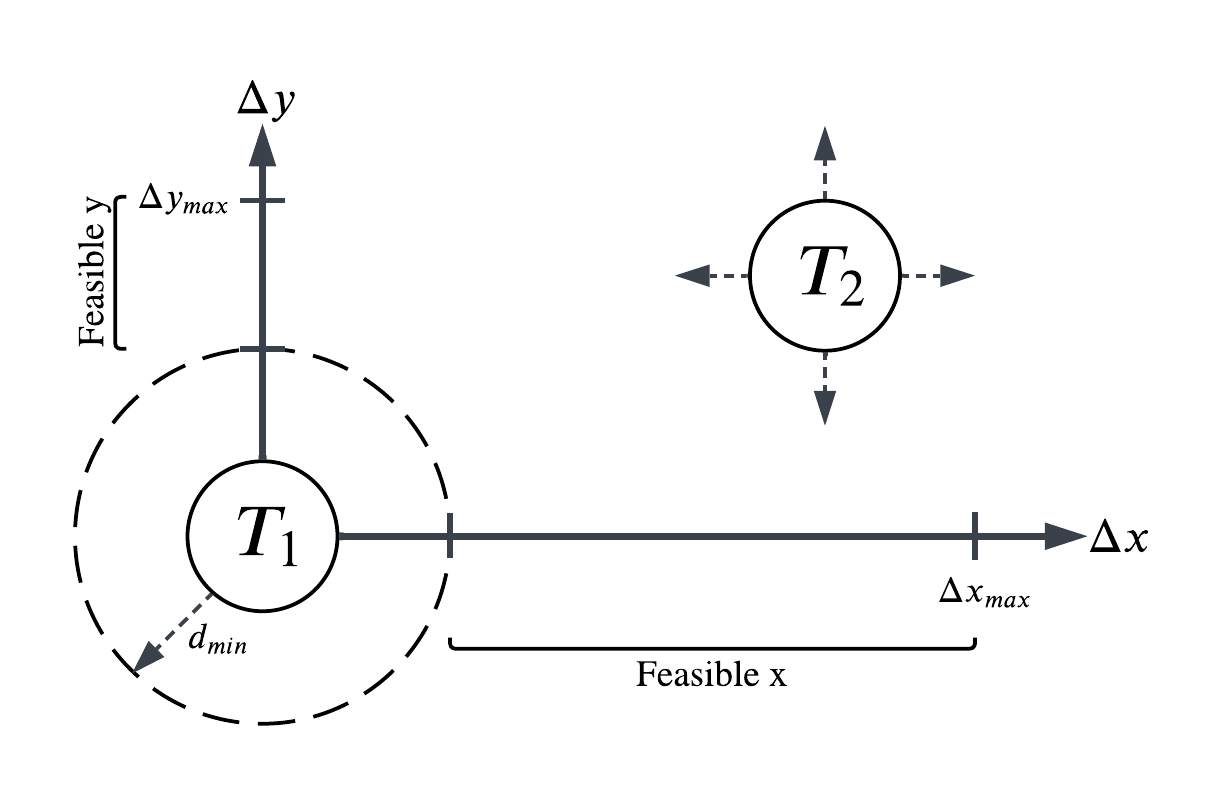
\includegraphics[width=0.6\textwidth]{figures/optimization/two_turbine_problem_schematic.png} % file name without extension
	\caption{Optimizing the relative position $\Delta x$/$\Delta y$ of a second wind turbine $T_2$ to a fixed first turbine $T_2$, constrained by minimum distance $d_{min}$ to  $T_1$ and maximum distances $\Delta x_{max}$/$\Delta y_{max}$}
	\label{fig:two_turbine_problem}
\end{figure}

The objective function to be optimized is the total power generation, e.g. the sum of power generated by both turbines. This objective is a function both of the position of the wind turbine as well as of the wind conditions like wind direction and wind speed. 

$$
f_{total Power}(x,y,\text{windspeed},\text{wind direction}, \text{(...)})
$$

Differently from the geographic coordinates, th wind condition parameters like windspeed are inherently not deterministic and follow distributions like the normal distribution as shown in Figure \ref{fig:wind_dist}.

\begin{figure}[h] 
	\centering
	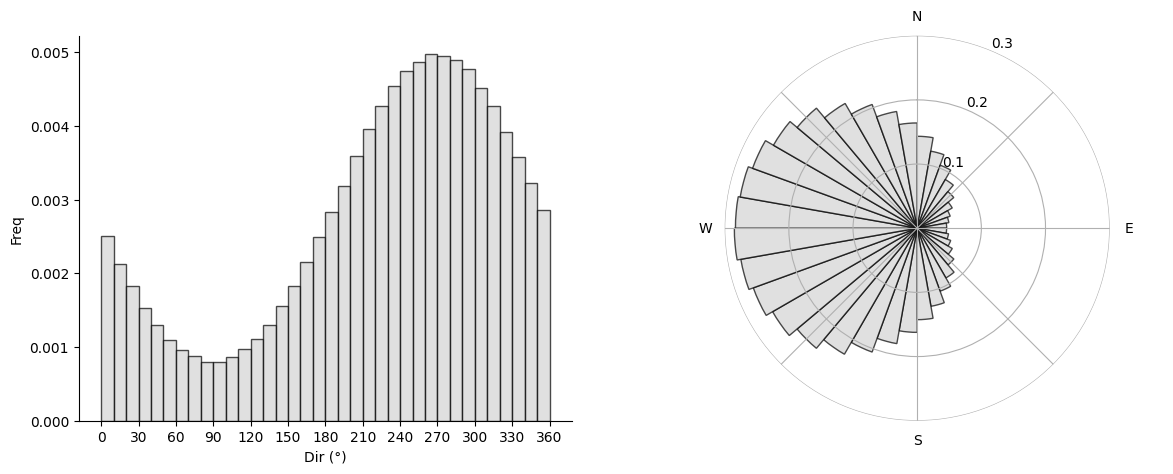
\includegraphics[width=0.9\textwidth]{figures/optimization/wind_dist.png} % file name without extension
	\caption{Histogram and Polar Plot across radiants for a normally distributed wind direction probability density function with mean West}
	\label{fig:wind_dist}
\end{figure}

The two main challenges of the optimization of the shown two turbine problem are thus: 

\begin{enumerate}
	\item Introduce the complex relationship between turbine position and wind conditions and power output into the optimization problem
	\item Introduce the non-deterministic nature of wind conditions into the optimization problem
\end{enumerate}

The first of these challenges is tackled by applying the Neural Network models discussed in Section \ref{sec:modelling} and introduce them into the optimization problem via constraint learning as described in Section \ref{sec:constraint_learning}. For the second problem, multiple approaches are now explored in the following subsection.


\subsection{Deterministic Optimization : Optimization for main Wind direction and Speed}

To begin with solving the problem, the most simplest approach is taken by assuming the wind conditions to be discrete. In application, this might be analouge to getting the Expectation of the joined probability distribution all wind condition parameters. Taking these parameters as constant and homogenious across the entire parameter space, the result is a objective function that is effectively only dependent on the relative positions of the turbine with the previously discussed geometrical constraints.

\begin{align}
	\max_{\mathbf{x}, \mathbf{y}} & f_{Power,\text{NN}}(\Delta x, \Delta y) \\
	\text{s.t.} \quad 
	&  \Delta x \leq X_{\max} \\
	&  \Delta y \leq Y_{\max} \\
	& \sqrt{(\Delta x)^2 + (\Delta y)^2} \geq d_{\min}
\end{align}

where:
\begin{itemize}
	\item \( (\Delta x, \Delta y) \) are the relative distances of the two turbines,
	\item \( f_{Power, \text{NN}}(\Delta x, \Delta y)\) is a neural network (deterministic) approximating the total power output ,
	\item \(  X_{\max}, Y_{\max} \) define the maximal distance the two turbines can be placed apart
	\item \( d_{\min} \) is the minimum distance between the two turbines.
\end{itemize}


When solving this problem as defined using Gurobi, a major challange becomes apparent as the result shows that there is an infinite amount of equally optimal solutions (e.g. degeneracy of the problem, see  \cite{vanderbei2020chapter3} for exact definition of degeneracy) everywhere outside the wake of turbine 1. This phenomenon is very intuitive when generating a heatmap of the power generation for all possible positions of turbine 2, as shown in Figure \ref{fig:two_turbine_heatmap_degeneracy}

TODO :  Insert Figure

%\begin{figure}[h] 
%	\centering
%	\includegraphics[width=0.9\textwidth]{figures/optimization/} 
%	\caption{}
%	\label{fig:two_turbine_heatmap_degeneracy}
%\end{figure}

This phenomenom whill have to be kept in mind going forwards, while introducing a distribution for wind condition parameters might reduce the number of global optima. 


\subsection{Stochastic Optimization:  Power weighted by probability}

As the deterministic optimization does not take into accound the distribution of wind condition parameters and having found that the deterministic approach leaves a range of infinite global optima outside of the wake of turbine 1, the next step is proceeding with the introduction of uncertainty in the form of probability distributions of wind condition parameters into the problem. This step primarily changes the objective function, which is set up such that the neural network takes in both position and wind condition parameters. the output of this neural network is then weighed by the probability of the specific wind condition occouring and the Expected power is calculated by integrating (discretized as sum) across all combinations of wind condition parameters.

\begin{align}
	\max_{\mathbf{x}, \mathbf{y}} &  \sum_{i=1}^{n} f_{Power,\text{NN}}(\Delta x, \Delta y, \text{wind condition})\cdot p_{n,\text{wind condtion combination}} \\
	\text{s.t.} \quad 
	&  \Delta x \leq X_{\max} \\
	&  \Delta y \leq Y_{\max} \\
	& \sqrt{(\Delta x)^2 + (\Delta y)^2} \geq d_{\min}
\end{align}

where:
\begin{itemize}
	\item \( (\Delta x, \Delta y) \) are the relative distances of the two turbines,
	\item \( f_{Power, \text{NN}}(\Delta x, \Delta y)\) is a deterministic neural network  approximating the total power output for turbine positions and wind conditions
	\item \(  X_{\max}, Y_{\max} \) define the maximal distance the two turbines can be placed apart
	\item \( d_{\min} \) is the minimum distance between the two turbines
	\item \( n \) is index of the discretized possible combinations of wind conditions 
	
In practice, this approach come with challenges as it requires the constraints representing the neural network to be realized $n$ times for each wind condition combination. With one instance of the neural network already adds a significant amount of constraints to the optimization model, realizing those constraints $n$ times may lead to an overflow of constraints, making the model to dificult to solve.
	
\subsection{Stochastic Optimization:  Power function as Quantile Neural Network}

An alternative approach to the one shown in the previous section, is to implant the uncertainties of the wind condition into the power model, with the output as quantiles from a quantile neural network. 


	
\end{itemize}

\section{The 3 turbine problem}

\section{The n turbine problem}

Thoughts: 

IDEA: generalize inputs in a way that allow for power calculation of each turbine individually instead of farm power

IDEA : derive basic rules from 2 turbine problem and set up new optimization problem without NN 

IDEA : analogue to forward/backward selection with 2 turbine neural network


FINIDINGS: 

problem degenerate if not one wind turbine fixed